\section{Introduction}
\label{sec:introduction}

\para{App flourish}. Mobile and Internet of Things (IoT) applications---such as
Microsoft SeeingAI~\cite{seeingai} and Google
Assistant~\cite{googleassistant}---are increasingly powered by machine learning
for daily tasks. These applications perform the \textit{inference} step of
machine learning: they use trained models to make a prediction given an input,
such as visual~\cite{googlelens, ha2014towards, seeingai}, audio~\cite{alexa,
  applesiri, cortana}, and sensory information~\cite{laput2017synthetic,
  lu2010jigsaw}. While there is a staggering collection of research focusing on
model \textit{training}, model deployment and prediction serving has received
relatively little attention.  In this paper, we study prediction serving for
wide-area mobile/IoT applications.

\para{Challenge to provide consistent low latency (sub-second) response}. Low
latency serving is important for smooth user experience. Previous
studies~\cite{nielsen1994usability, schneiderman1998designing} have measured the
effect of different end-to-end latencies: 100 ms gives the feeling of
instantaneous response, 1 second keeps the user's flow of thought seamless, and
a few seconds' delay creates an unpleasant user experience.

%% Reference:
%% https://www.nngroup.com/articles/website-response-times/

%% 0.1 seconds gives the feeling of instantaneous response — that is, the
%% outcome feels like it was caused by the user, not the computer. This level of
%% responsiveness is essential to support the feeling of direct manipulation
%% (direct manipulation is one of the key GUI techniques to increase user
%% engagement and control — for more about it, see our User Interface Principles
%% Every Designer Must Know course).

%% 1 second keeps the user's flow of thought seamless. Users can sense a delay,
%% and thus know the computer is generating the outcome, but they still feel in
%% control of the overall experience and that they're moving freely rather than
%% waiting on the computer. This degree of responsiveness is needed for good
%% navigation.

%% 10 seconds keeps the user's attention. From 1–10 seconds, users definitely
%% feel at the mercy of the computer and wish it was faster, but they can handle
%% it.

%% There are also some great discussion about latency here:
%% https://danluu.com/term-latency/

%% More examples: Wearable cognitive assistant~\cite{ha2014towards} that uses
%% wearable devices, such as Google Glass, for deep cognitive assistance (e.g.,
%% offering hints for social interaction via real-time scene analysis).
%% SeeingAI is a talking camera for the blind and low vision community that
%% describes nearby people, text, objects. \xin{Google lens
%% (https://36kr.com/p/5075676.html).  Siri, Google assistant, Amazon Alexa
%% (Echo).}

\para{Why challenging? Discrepancy in performance, shared network/service.}
Meeting sub-second latency goals consistently has remained challenging,
especially for complex prediction servings beyond the capabilities of end
devices. State-of-the-art computer vision algorithms, such as object detection,
easily take several seconds on modern smartphones~\cite{chen2015glimpse}. Prior
work explores offloading to the cloud or the edge\footnote{Also referred to as
  cloudlet~\cite{satyanarayanan2009case}, the fog~\cite{bonomi2012fog}.}  that
hosts machine learning models and serves predictions. Despite their powerful
computing capability and more available resources---including special hardware
like GPU and TPU~\cite{jouppi2017datacenter}---these platforms suffer from
increased network latency and service overload, thus unable to meet latency
goals consistently. We illustrate the spectrum of resources, workload and
latency among end devices, the edge and the cloud in
\autoref{fig:mobile-edge-cloud}.

%% Existing systems~\cite{crankshaw2017clipper, yun2015optimal} strives to bound
%% tail performance to meet service level objectives (SLO).

\begin{figure}
  \centering
  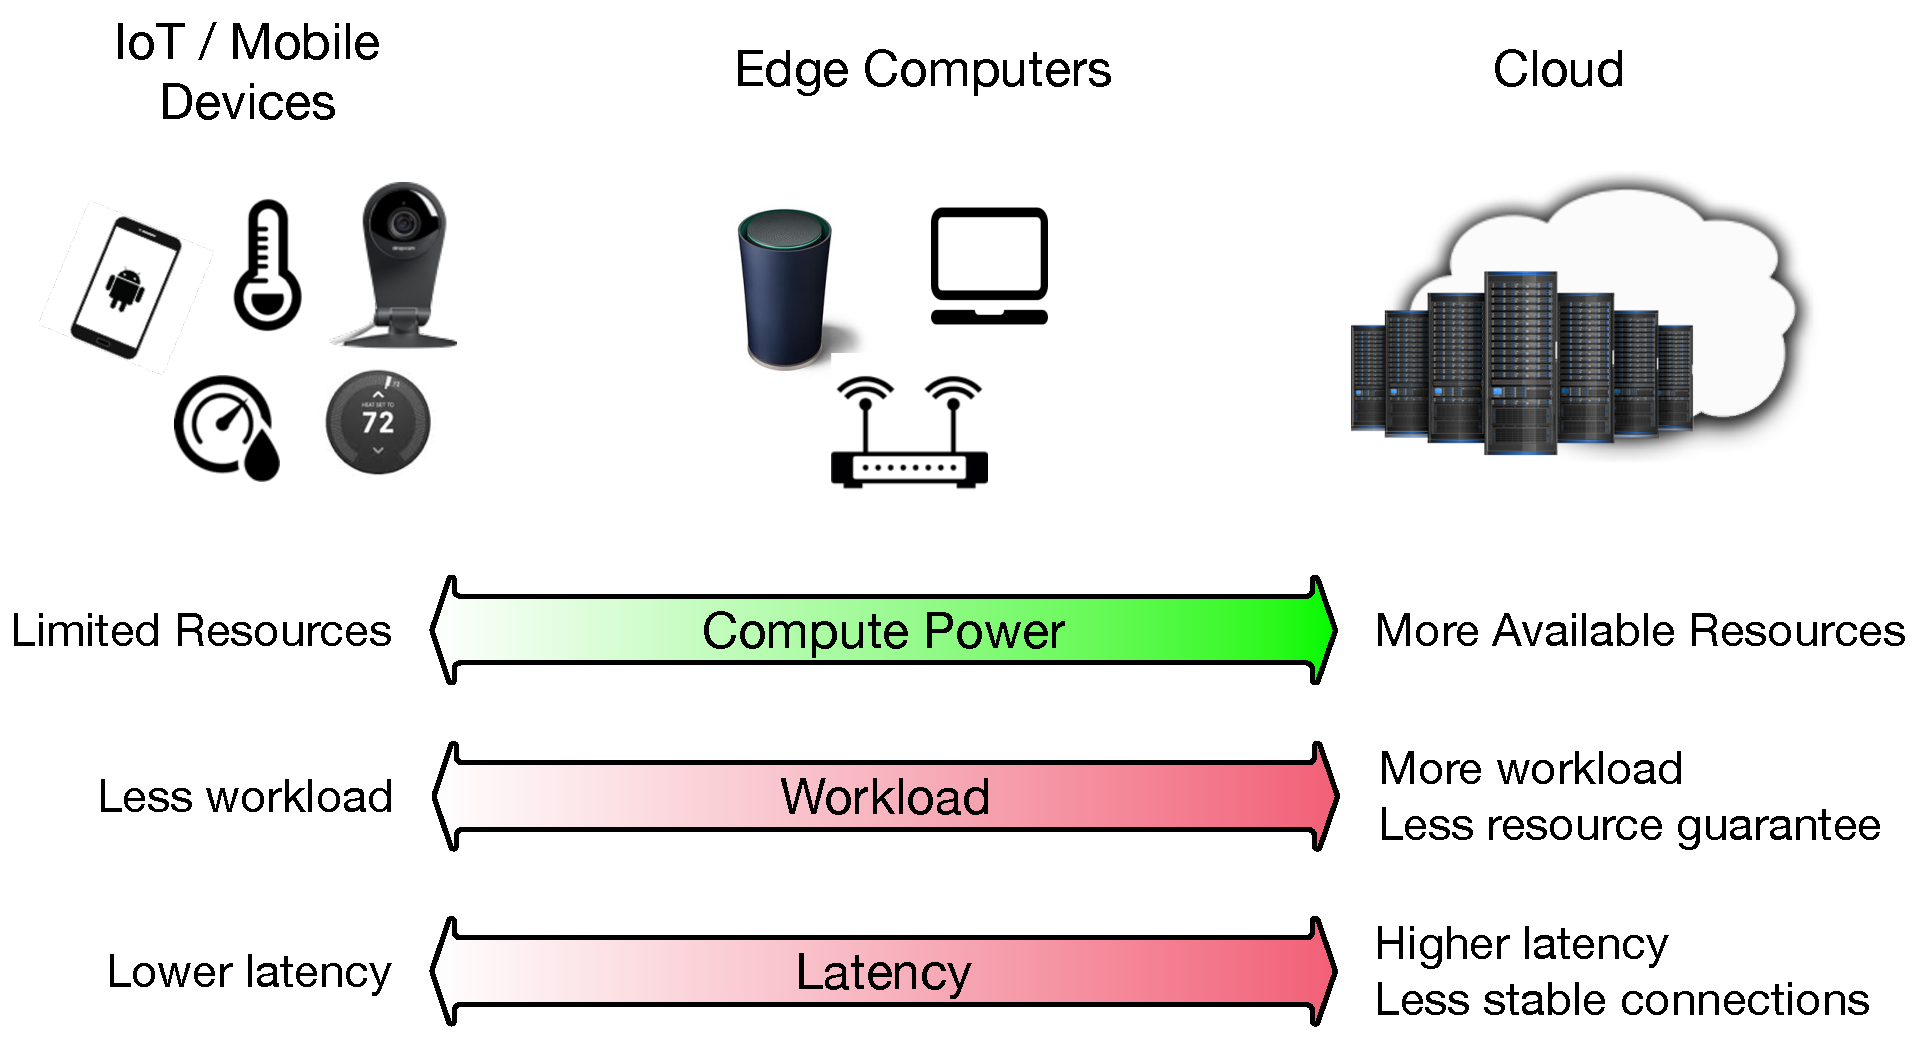
\includegraphics[width=0.95\columnwidth]{figures/background.pdf}
  \caption{Characteristics of IoT/mobile, edge and cloud.}
  \label{fig:mobile-edge-cloud}
\end{figure}

This paper presents \sysname{}, a general prediction serving framework that
provides bounded response times for IoT. Its core is about performance modeling
by exploring the tradeoff space between application accuracy and cost
(processing times). Orthogonal to existing system solutions with scale-out,
scale-up, caching or batching, \sysname{} requires knowledge from the
application.

\para{(short) Accuracy-Cost Tradeoff.} For a particular inference task, multiple
algorithms or tunable parameters for one algorithm exist that requires different
processing times and result in different accuracy. To accommodate the
resource-constrained devices, one can use an algorithm or a parameter that suits
the particular platform. In order to explore the trade-off space, \sysname{}
takes a data-driven approach to learn the relationship between inference
accuracy and processing times for each algorithm and different parameters for
individual platforms. We call this process ``profiling'' and its goal is to find
Pareto-optimal configurations (algorithm and parameter) as the performance
model. Profiling with an exhaustive search may not be feasible for some
algorithms due to their large parameter space. In these cases, \sysname{} uses a
statistical method, Bayesian Optimization (BO), to model the relationship as a
black-box function and only searches for near-optimal configurations.

\para{(short) Ensemble of Machines.} While running a low accuracy configuration
on end devices ensures bounded latency, the accuracy may not be
satisfactory. \sysname{} improves the accuracy by combining available resources
such as the edge and the cloud, similar to existing techniques such as
offloading~\cite{chun2011clonecloud,cuervo2010maui} and redundant
requests~\cite{ananthanarayanan2013effective, dean2013tail,
  gordon2015accelerating, vulimiri2013low}. One key difference between
\sysname{} and existing approaches is that \sysname{} uses the learned
performance model to find platform-specific configurations instead of running
the same computation (\autoref{fig:dr}).

\begin{figure}
  \centering
  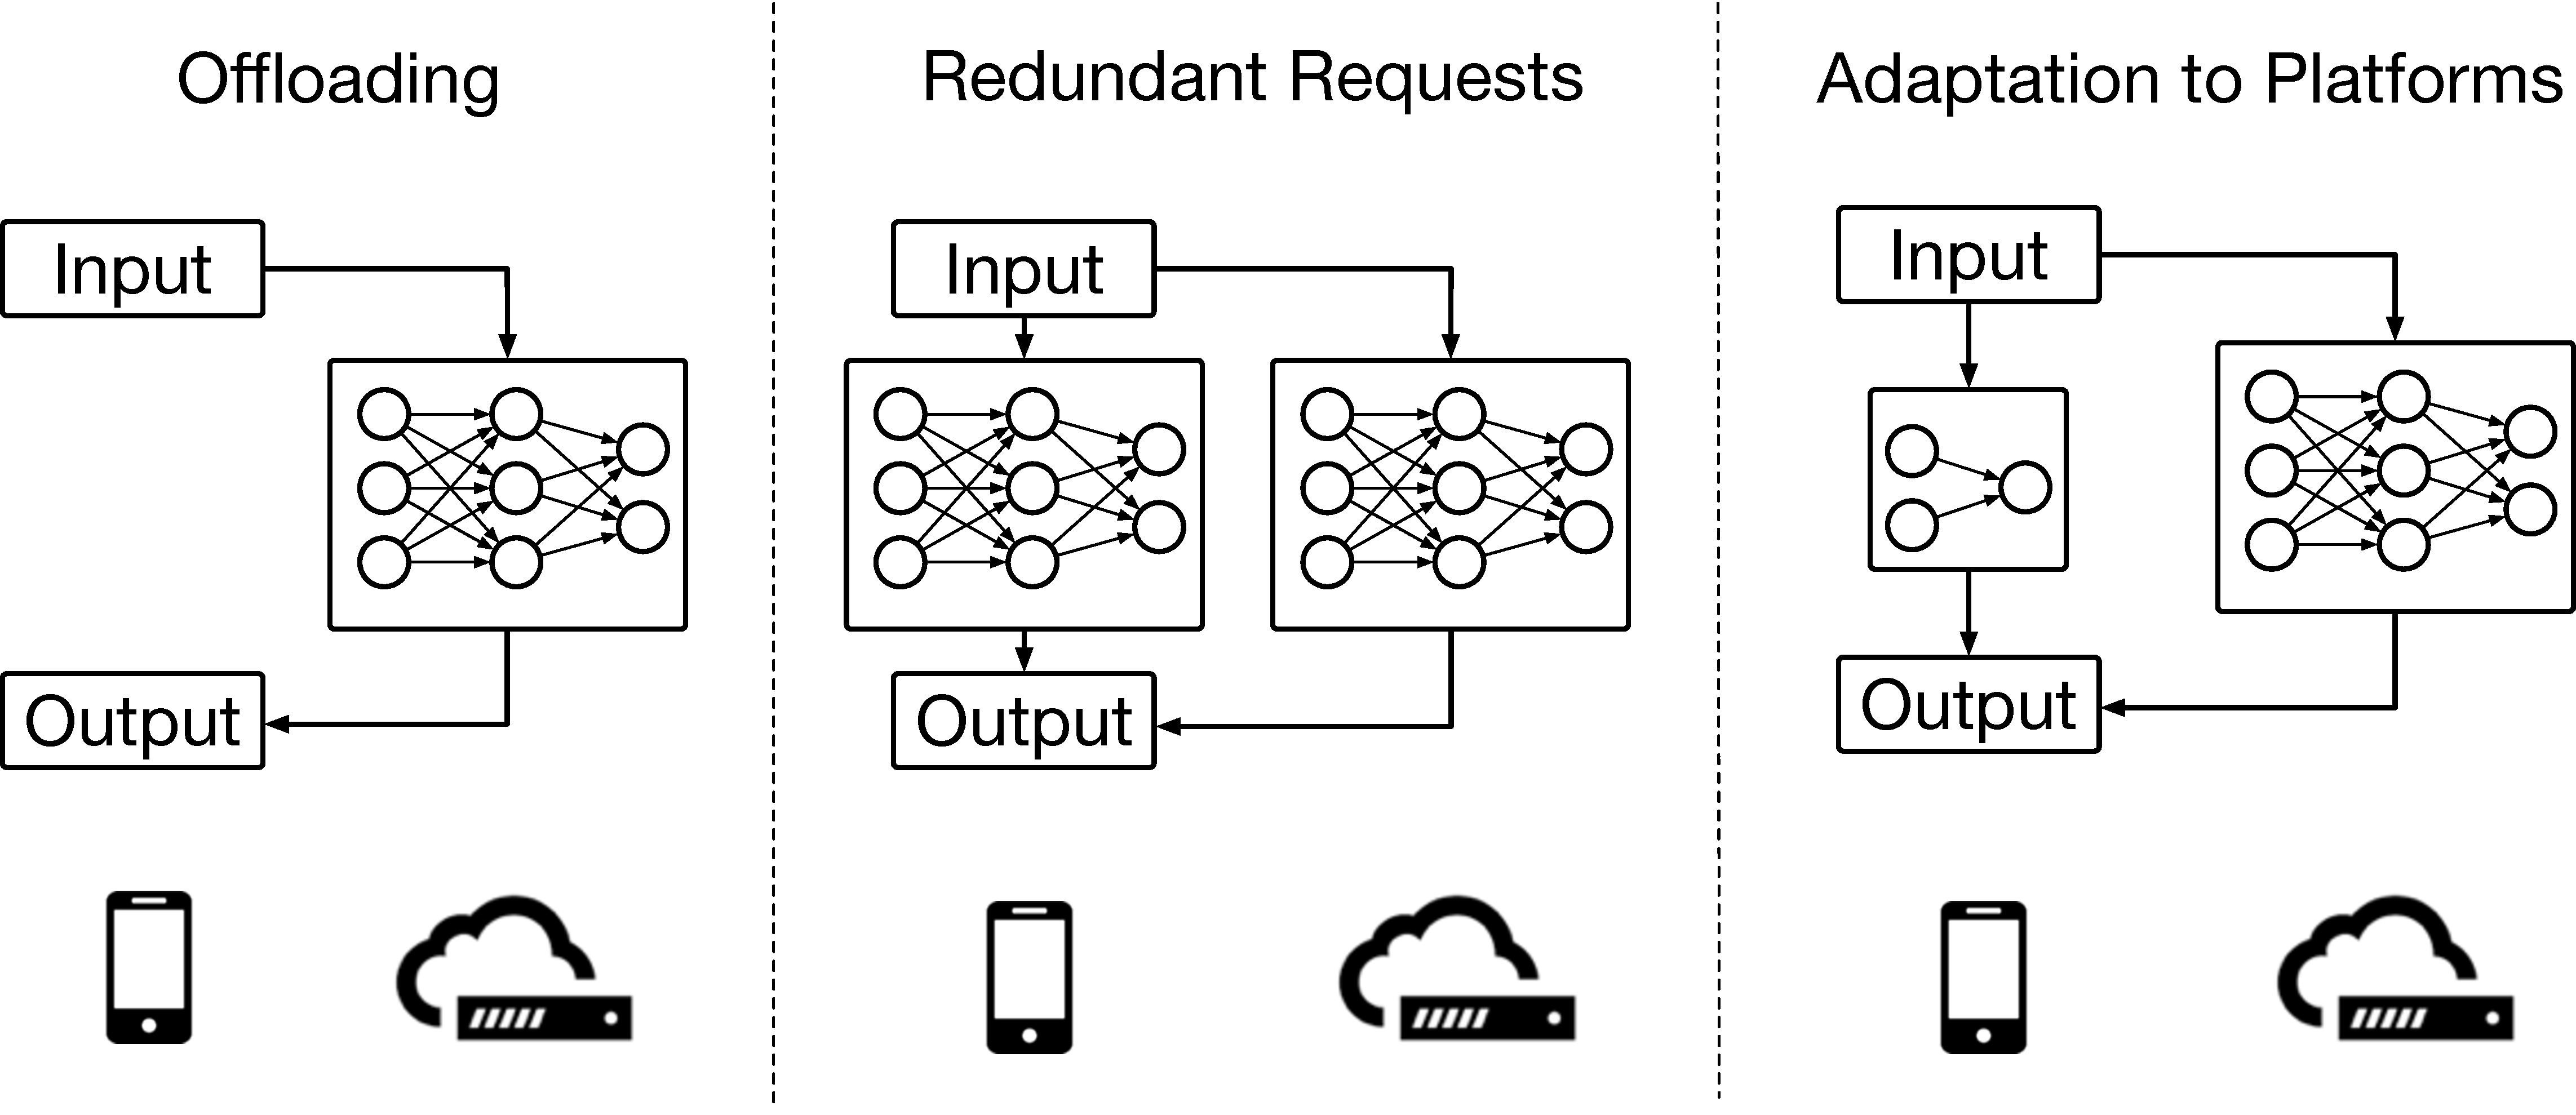
\includegraphics[width=\columnwidth]{figures/dr.pdf}
  \caption{Illustration of offloading, redundant requests and differential
    redundancy.}
  \label{fig:dr}
\end{figure}

We call this differential differential redundancy (DR) and illustrate the idea
using face detection as an example. For a particular image, a less power
platform, such as the mobile, can reduce the image resolution to speed up
detection. As a result, it only detects large faces, offering an
inaccurate-but-fast response. At the same time, a redundant request is sent to a
powerful server. The server can detect all tiny faces, yielding a higher
accuracy. The result is then returned and merged with the initial result. From
the user's perspective, face detection is \emph{instantaneous} and gradually
\emph{accurate}.

To make DR effective and efficient, \sysname{} should utilize available
resources but avoid sending unnecessary requests. We treat the as a multi-armed
bandit problem and model the uncertainty behind network delays and service
contention. When the uncertainty grows, it favors redundant requests
(exploration); if there is an apparent winner among all dispatching options, it
avoids excessive service requests (exploitation).

\para{(short) SLO-aware scheduling.} Each request is annotated with a
service-level objective (SLO) that describes the deadline and accuracy
demand. Upon receiving a request, the server runs a real-time scheduler to meet
all SLOs. Existing real-time scheduler often assumes a worst-case execution time
(WCET) and runs earliest deadline first (EDF) schedule. Our scheduler has two
key differences when trying to meet SLOs: $(i)$ \sysname{} can adjust each
request's serving time and quality based on the profile; $(ii)$ \sysname{} is
allowed to reject a request because of the redundancy mentioned above.

At runtime, when a request comes in, the server first performs triage to
determine the urgency of the request and its priority among all pending
tasks. If all tasks are still schedulable after admitting the new request, it's
added to the task queue; otherwise, \sysname{} rejects the request. The
schedulability is checked if all requests are serviced at its lowest-allowed
quality; this allows us to reject fast by only keeping track of available
\texttt{capacity}. When performing the actual scheduling, \sysname{} can spare
the remaining capacity to increase some tasks' quality. Our scheduler is
non-preemptive and treat all requests equally.

We've implemented the aforementioned techniques and evaluated their
effectiveness over three applications. We make the following contributions with
\sysname{}:

\begin{itemize}[leftmargin=*, topsep=0pt, itemsep=0pt]

\item Performance modeling. We cast the performance modeling as multi-objective
  optimization problems. Our BO-based profiling can effectively explore the
  large parameter space and finds near-optimal solutions.

\item Differential redundancy. For prediction serving, we propose to use perform
  redundant servings with different algorithms and parameters for each platform
  to harness the heterogeneity.

\item Runtime dispatch. During the runtime dispatch, we model the online
  scheduler as a multi-armed bandit problem with budget constrain. Our scheduler
  is able to save 30\% energy over baseline schedulers.

\item Server triage. The server continuously adjusts the priority of each
  requests to maximize throughput while meeting SLOs.

\end{itemize}

% \begin{figure*}
%   \centering
%   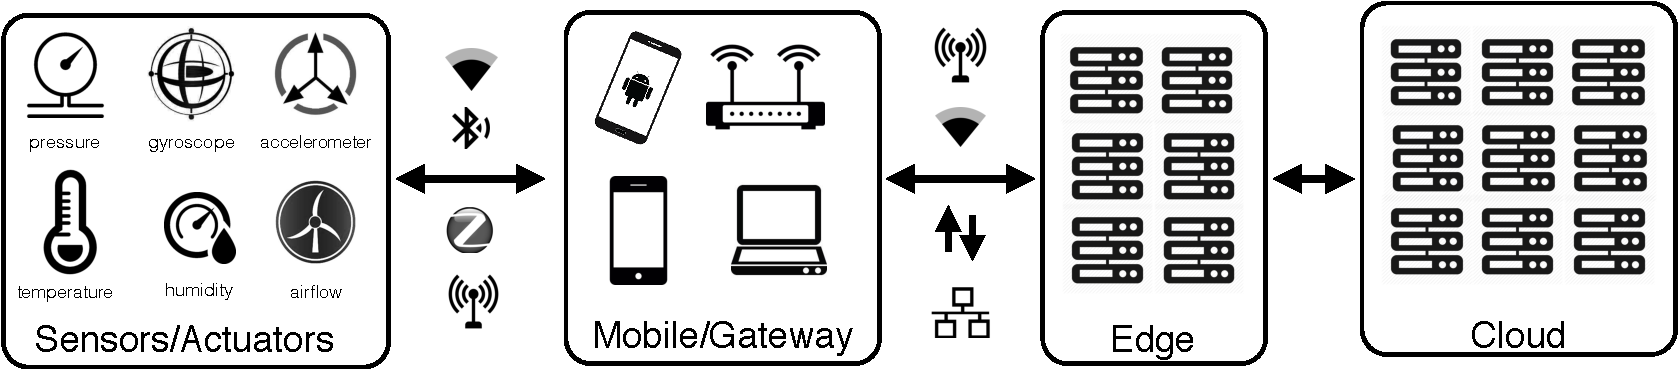
\includegraphics[width=\textwidth]{figures/platforms}
%   \label{fig:options}
%   \caption{Platforms}
% \end{figure*}

%%% Local Variables:
%%% mode: latex
%%% TeX-master: "../../thesis"
%%% End:
